% =====================================================================
%  Paper final — Optimización 1 (EAFIT), 2026-2
%  Focalización del gasto para reducir el IPM en Antioquia:
%  información perfecta, geográfica y mixta (Modelos 1-4)
%
%  Compilar:  latexmk -pdf main.tex      (o subir la carpeta a Overleaf)
%  Regla de oro: cada quien edita SOLO sus archivos de secciones/
%  (el responsable está en la primera línea de cada archivo).
%  Las cifras van en cifras.tex, nunca escritas a mano en el texto.
% =====================================================================
\documentclass[11pt,a4paper]{article}

\usepackage[utf8]{inputenc}
\usepackage[T1]{fontenc}
\usepackage{lmodern}
% Español si está instalado (Overleaf y TeX Live completo lo tienen);
% si no, compila igual con nombres en español puestos a mano.
\IfFileExists{spanish.ldf}{%
  \usepackage[spanish,es-noshorthands,es-tabla]{babel}%
}{%
  \usepackage[english]{babel}%
  \addto\captionsenglish{%
    \renewcommand{\abstractname}{Resumen}%
    \renewcommand{\refname}{Referencias}%
    \renewcommand{\tablename}{Tabla}%
    \renewcommand{\figurename}{Figura}%
    \renewcommand{\appendixname}{Apéndice}%
    \renewcommand{\contentsname}{Contenido}}%
}
\usepackage[margin=2.5cm]{geometry}
\usepackage{amsmath,amssymb,amsthm}
\usepackage{icomma}            % coma decimal en modo matemático: $0,0387$
\usepackage{booktabs,tabularx,multirow}
\usepackage{graphicx}
\graphicspath{{figuras/}}
\usepackage[dvipsnames]{xcolor}
\usepackage{caption,subcaption}
\usepackage[round,authoryear]{natbib}
\usepackage[hidelinks]{hyperref}

% --- Marcas de trabajo pendiente (se ven en rojo en el PDF) -----------
% Para la versión de entrega: cambiar \borradortrue por \borradorfalse.
\newif\ifborrador \borradortrue
\ifborrador
  \newcommand{\pendiente}[1]{{\color{BrickRed}\textbf{[PENDIENTE:} #1\textbf{]}}}
  \newcommand{\nota}[2]{{\color{NavyBlue}\textbf{[#1:} #2\textbf{]}}}
\else
  \newcommand{\pendiente}[1]{}
  \newcommand{\nota}[2]{}
\fi

\newtheorem{proposition}{Proposición}

% Responsable: Jerónimo (notación común; Martín puede agregar macros de M1/M2 al final)
% Una sola notación para los 4 modelos. Si necesitas un símbolo nuevo,
% agrégalo aquí y en la Tabla de notación (secciones/04_notacion_comun.tex).

% --- Conjuntos e índices ---
\newcommand{\Hog}{\mathcal{I}}        % hogares, i
\newcommand{\Ind}{\mathcal{J}}        % indicadores, j
\newcommand{\Zon}{\mathcal{D}}        % celdas geográficas (zonas), d
\newcommand{\Tip}{\mathcal{T}}        % tipos de hogar (clústeres), t
\newcommand{\Upriv}{\mathcal{U}}      % indicadores de bien privado (M4)
\newcommand{\Vpub}{\mathcal{V}}       % indicadores de bien público (M4)

% --- Parámetros ---
\newcommand{\HS}{HS}                  % tamaño del hogar
\newcommand{\HW}{HW}                  % factor de expansión
\newcommand{\EpF}{EpF}                % costo unitario de quitar una privación
\newcommand{\MPIs}{M_0^{s}}           % M0 inicial
\newcommand{\MPIr}{m}                 % meta de reducción de M0 (12-nov: m, no r; r es el piso por zona)

% --- Variables ---
\newcommand{\Ndec}{N}                 % privación después de intervenir (binaria)
\newcommand{\Esf}{E}                  % esfuerzo (gasto)
\newcommand{\Cont}{C}                 % contribución del hogar al M0 final
\newcommand{\cob}{\theta}             % cobertura de un par (j, celda) (12-nov: theta, no p)

% --- Operadores ---
\newcommand{\Mcero}{M_0}
   % macros de notación común a los 4 modelos
% Responsable: cada quien sus cifras (bloques separados para no chocar).
% REGLA: toda cifra del texto sale de aquí y cada macro dice de qué CSV viene.
% Si se repite una corrida, se cambia SOLO aquí y el paper queda coherente.
% Formato: coma decimal, punto de miles (como en las diapositivas).

% ===== Línea base (Martín) =============================================
% Fuente: Modelos/04_linea_base.py
\newcommand{\cMcero}{0,0387}          % M0 inicial (exacto: 0,038684)
\newcommand{\cHogares}{3.732}         % hogares de Antioquia en la muestra
\newcommand{\cIndicadores}{15}
\newcommand{\cMceroExacto}{0,038684}
\newcommand{\cPobresHog}{523}           % hogares pobres en la línea base
\newcommand{\cHcero}{9,45\,\%}         % verificado en CLAUDE.md de Modelo3 §3
\newcommand{\cAcero}{40,94\,\%}

% ===== Modelos 1 y 2 (Martín) ==========================================
% Fuente: \pendiente{CSV de resultados M1/M2 en el escenario común}

% ===== Modelos 3 y 4 (Jerónimo) ========================================
% Tamaño del modelo en la VERSIÓN INICIAL (costos por persona, meta 10 %, réplica 0). Fuente: docs_proyecto/revision-formulacion-modelo3.md
% y CLAUDE.md de Modelo3 §3 y §5 (meta 10 %, réplica 0)
\newcommand{\cParesActivos}{8.602}     % pares (i,j) con M_ij = 1
\newcommand{\cParesMtres}{45}          % pares (indicador, zona), versión inicial (con rezago)
\newcommand{\cParesMcuatro}{53}        % pares (indicador, celda) en M4, escenario final (m34_tamano_modelo.py)
\newcommand{\cCortesMtres}{630}
\newcommand{\cCortesMcuatro}{324 y 524}   % escenario final, 100 réplicas
\newcommand{\cBinPaper}{171.672}      % Lin 6-10 literal, b1 para todos los hogares
\newcommand{\cBinDirecta}{9.125}       % N = b2 y b1 solo para pobres: 8.602 + 523
\newcommand{\cRestrDirecta}{27.376}
\newcommand{\cBinCortes}{1.153}
\newcommand{\cRestrCortes}{1.615}
\newcommand{\cTiempoCortes}{2,1~s}
% Escenario final (datos-finales-10nov), 100 réplicas. Fuente: m34_tamano_modelo.py
\newcommand{\cParesMtresFin}{42}
\newcommand{\cCortesMtresFin}{318 y 542}
\newcommand{\cBinMtresFin}{841 a 1.065}
\newcommand{\cTiempoMtresMed}{1~s}
\newcommand{\cTiempoMtresMax}{22~s}
\newcommand{\cLogroFijos}{1.647}       % pares de logro que el M1 no puede quitar en un año
% Modelo 4. Fuente: CLAUDE.md de Modelo3 §8 y §7.4 (clústeres no dependen de los costos)
\newcommand{\cDiscAcuZona}{14,5}
\newcommand{\cDiscAcuClu}{4,1}
\newcommand{\cSeparaPobreza}{4,3}
\newcommand{\cSiluetaMin}{0,26}
\newcommand{\cSiluetaMax}{0,28}
\newcommand{\cDiscInasClu}{51,7}
\newcommand{\cHcabecera}{6,2\,\%}          % H0 de la cabecera, CLAUDE.md de Modelo3 §3
% Validación del escenario común contra el M1/M2 de main (10-nov). Fuente: resultados/m34/validacion_10nov.csv
\newcommand{\cValidOK}{18 pruebas}
\newcommand{\cParesPobres}{2.592}
\newcommand{\cVcincoVeinte}{5,9\,\%}
\newcommand{\cVcincoTreinta}{2,7\,\%}
% Validación 12-nov (granularidad máxima con meta por zona y r_B). Fuente: resultados/m34/validacion_12nov.csv
\newcommand{\cGunoTreinta}{0,4\,\%}
\newcommand{\cGdosMin}{0,3}
\newcommand{\cGdosMax}{1,0\,\%}
% Corridas del 10-nov (escenario común contra el M1/M2 de main), CONGELADAS. Fuente: resultados/m34/*_10nov.csv
% en la rama Modelo3, etiqueta datos-finales-10nov. Costos: 100 réplicas; equidad: 100 (B <= 10) y 30 (B >= 25).
\newcommand{\cReplicas}{30}               % equidad con B >= 25
\newcommand{\cReplicasCosto}{100}
\newcommand{\cCorridasCosto}{4.500}
\newcommand{\cMtresIPmin}{6}
\newcommand{\cMtresIPmax}{17}
\newcommand{\cMtresIPalta}{3,5 a 3,9}
\newcommand{\cMcuatroPlacMin}{14\,\%}
\newcommand{\cMcuatroPlacMax}{31\,\%}
\newcommand{\cReplicasBajo}{100}
\newcommand{\cMtresPctMin}{13\,\%}
\newcommand{\cMtresPctMax}{65\,\%}
\newcommand{\cMcuatroPlacEq}{9--10\,\%}
\newcommand{\cInfactiblesRho}{900}
% ===== Comparación principal (12-nov): restricciones de equidad de Martín tal cual =====
% Criterio de costo con meta de M0 en cada zona. Fuente: resultados/m34/costo_meta_zona_crudo_12nov.csv e
% ic_costo_meta_zona_12nov.csv (m34_tablas_12nov.py); IP = info_perfecta_meta_zona_12nov.csv (M2 sin E-7).
\newcommand{\zReplicas}{54}
\newcommand{\zCorridas}{2.430}
\newcommand{\zGapMax}{$8{,}8\times10^{-7}$}
\newcommand{\zMtresIPmin}{3,2}            % M3/IP, mínimo (meta 28 %)
\newcommand{\zMtresIPmax}{12,5}           % M3/IP, máximo (meta 2 %)
\newcommand{\zMtresIPbaja}{5,5 a 12,5}    % metas del 2 al 10 %
\newcommand{\zMtresIPalta}{3,2 a 3,9}     % metas del 20 al 30 %
\newcommand{\zMcuatroIPmin}{3,4}
\newcommand{\zMcuatroIPmax}{8,3}
\newcommand{\zMcuatroMtresMenor}{5}       % metas con IC de M4/M3 < 1 (2, 12, 20, 22, 24 %)
\newcommand{\zMcuatroMtresMayor}{2}       % metas con IC de M4/M3 > 1 (28, 30 %)
\newcommand{\zMcuatroMtresIgual}{8}
\newcommand{\zPlacMin}{14\,\%}            % M4 más barato que el placebo, desde la meta del 6 %
\newcommand{\zPlacMax}{37\,\%}
\newcommand{\zInclMtres}{27 y 55\,\%}     % inclusión mediana por meta, M3
\newcommand{\zInclMcuatro}{21 y 49\,\%}
\newcommand{\zExclMtres}{56 y 93\,\%}
\newcommand{\zIPzonaDiez}{5,17}           % IP (M2) con meta del 10 % por zona
\newcommand{\cIPglobalDiez}{1,32}         % IP (M2) con meta global del 10 % (10-nov)
% Criterio de cobertura con r_B. Fuente: resultados/m34/cobertura_rB_crudo_12nov.csv y rmax_12nov.csv
% (m34_rmax_12nov.py; ic_rmax_12nov.csv con m34_tablas_12nov.py), 100 réplicas.
\newcommand{\zCorridasCob}{1.350}           % 1.170 con r_B y 180 con r_B y rho_B (B = 25 y 50)
\newcommand{\zCorridasRmax}{1.800}
\newcommand{\zRmaxFracMin}{0}             % r_max(M3)/r_max(IP), mediana, B = 2
\newcommand{\zRmaxFracMax}{56\,\%}        % B = 100
     % TODAS las cifras del paper, con su CSV de origen

\title{Focalización del gasto público para reducir la pobreza multidimensional
en Antioquia: el costo de no saber quién es pobre%
\thanks{Proyecto final de Optimización 1, Universidad EAFIT.
Adaptación de los Modelos 1--4 de \citet{hamie2024}.}}
\author{Martín Quijano \and Jerónimo Vélez\\[2pt]
\small Ingeniería de Sistemas, Universidad EAFIT}
\date{Noviembre de 2026}

\begin{document}
\maketitle

% Responsable: AMBOS — se escribe de último (martes en la mañana)
% 200-250 palabras: problema, qué hicimos (4 modelos, datos IPM 2025 Antioquia),
% hallazgo principal (el precio de la información) y para qué sirve.
\begin{abstract}
\pendiente{Resumen de 200--250 palabras. Escribir al final.}

\medskip\noindent\textbf{Palabras clave:} pobreza multidimensional, Alkire--Foster,
programación lineal entera mixta, focalización, Monte Carlo, \emph{clustering}.
\end{abstract}


% Responsable: Martín (investigación y contexto)
% Tesis: el Estado colombiano focaliza con información imperfecta; la pregunta
% del paper es cuánto cuesta esa imperfección y cómo se reparte el gasto.
\section{Introducción}\label{sec:intro}

\pendiente{Contexto: IPM oficial en Colombia y Antioquia (cifras DANE 2025).}

\pendiente{Problema: el gasto social se asigna sin saber exactamente quién es
pobre (errores de inclusión y exclusión).}

\pendiente{Aporte: adaptamos los cuatro modelos de \citet{hamie2024} a Antioquia
y medimos el costo de pasar de información perfecta (Modelos 1--2) a
focalización geográfica (Modelo 3) y mixta (Modelo 4).}

\pendiente{Pregunta de investigación y estructura del documento
(Sección~\ref{sec:literatura} a Sección~\ref{sec:conclusiones}).}

% Responsable: Martín (investigación)
% 10-15 fuentes. Cada subsección termina diciendo qué hueco llena este trabajo.
\section{Revisión de literatura}\label{sec:literatura}

\subsection{Medición multidimensional de la pobreza}
\pendiente{Alkire--Foster \citep{alkire2011}; IPM de Colombia \citep{angulo2016};
brecha normalizada / severidad.}

\subsection{Focalización y errores de inclusión y exclusión}
\pendiente{\citet{coady2004}; SISBÉN IV y focalización geográfica en Colombia.}

\subsection{Optimización aplicada a la reducción de pobreza}
\pendiente{\citet{hamie2024} y trabajos relacionados (MILP, asignación de presupuesto).}

\subsection{Tipologías de hogares mediante \emph{clustering}}
\pendiente{k-medoides / PAM \citep{kaufman1990}; uso en encuestas de hogares.}
\nota{Jerónimo}{Martín: esta subsección sostiene el Modelo 4. Si no alcanzas,
la escribo yo con lo de la elección de $k$.}

\section{Método}\label{sec:metodo}
% Responsable: Martín (datos, línea base y costos)
% Fuentes en el repo: docs/informe_modelo1.md §2 y §6, docs/reglas_conteo_personas.md,
% docs/resumen_proyecto_ipm.md, Modelos/04_linea_base.py, Modelos/parametros.py
\subsection{Datos e índice de pobreza multidimensional}\label{sec:datos}

\pendiente{Fuente: microdatos DANE (IPM 2025), Antioquia, \cHogares{} hogares,
\cIndicadores{} indicadores, 3 zonas (P3). Ver la decisión de fuente de datos.}

\pendiente{Medida Alkire--Foster: puntaje, umbral $k=1/3$, $H$, $A$, $\Mcero$.
Línea base: $\Mcero = \cMcero$, $H = \cHcero$, $A = \cAcero$.}

\pendiente{Costos por indicador ($\EpF_j$) y unidad de pago $u_{ij}$
(detalle en el Apéndice~\ref{app:costos}).}

% Responsable: Jerónimo (relación entre los 4 modelos)
% Tesis: los 4 modelos son el MISMO problema con distinta información sobre
% quién es pobre. Esta tabla es el contrato: nadie usa otra notación.
\subsection{Notación común y jerarquía de información}\label{sec:notacion}

Los cuatro modelos comparten los datos, la medida de pobreza y la meta; lo único
que cambia entre ellos es \emph{qué sabe el planificador} sobre cada hogar en el
momento de asignar el gasto. Para que esa diferencia sea la única, todos se
escriben con la notación de la Tabla~\ref{tab:notacion}, que adapta la de
\citet[Tablas A1--A3]{hamie2024}.

\begin{table}[ht]
\centering\small
\caption{Notación común a los cuatro modelos.}\label{tab:notacion}
\begin{tabularx}{\textwidth}{@{}llX@{}}
\toprule
Símbolo & Tipo & Significado \\
\midrule
\multicolumn{3}{@{}l}{\emph{Conjuntos}}\\
$i\in\Hog$, $j\in\Ind$ & & hogares (\cHogares) e indicadores (\cIndicadores) \\
$\Hog^0\subseteq\Hog$ & & hogares pobres en la línea base (\cPobresHog) \\
$d\in\Zon$ & & zonas geográficas: cabecera, centro poblado, rural disperso \\
$t\in\Tip$ & & tipos de hogar obtenidos por \emph{clustering} (Modelo 4) \\
$\Ind=\Upriv\cup\Vpub$ & & indicadores de bien privado y de bien público (Modelo 4) \\
$g(i,j)$ & & celda de focalización del par $(i,j)$: $d_i$ en M3; $d_i$ o $t_i$ en M4 \\
\midrule
\multicolumn{3}{@{}l}{\emph{Parámetros}}\\
$w_j$, $k$ & & peso del indicador ($\sum_j w_j=1$); umbral de pobreza ($k=1/3$) \\
$M_{ij}\in\{0,1\}$ & & privación inicial del hogar $i$ en el indicador $j$ \\
$\HS_i$, $\HW_i$ & & tamaño del hogar; factor de expansión \\
$u_{ij}$ & & personas del hogar que hay que atender para quitar la privación \\
$c_{ij}$ & & costo de quitar la privación $(i,j)$ en un hogar de la muestra \\
$V_{ij}=u_{ij}\HW_i$ & & cobertura que aporta el par, en personas de la población \\
$K_{ij}=c_{ij}\HW_i$ & & gasto que exige el par, expandido a la población \\
$R_{ij}\sim U[0,1]$ & & sorteo fijo del par, independiente entre pares (M3--M4) \\
$\MPIs$, $\MPIr$ & & $\Mcero$ de la línea base (\cMceroExacto); reducción exigida \\
$B$ & & presupuesto (objetivo de equidad) \\
\midrule
\multicolumn{3}{@{}l}{\emph{Variables}}\\
$\Ndec_{ij}\in\{0,1\}$ & & privación después de intervenir ($\Ndec_{ij}\le M_{ij}$) \\
$s_i$ & & puntaje de privación final, $s_i=\sum_j w_j\Ndec_{ij}$ \\
$b1_i\in\{0,1\}$ & & $b1_i=1$ si y solo si el hogar \emph{sale} de la pobreza ($s_i<k$) \\
$\Cont_i\ge 0$ & & contribución del hogar al $\Mcero$ final \\
$\Esf_{jg}$ & & gasto en el indicador $j$ dentro de la celda $g$ \\
$\cob_{jg}\in[0,1]$ & & cobertura del par $(j,g)$: fracción de la población privada atendida \\
\bottomrule
\end{tabularx}
\end{table}

Con información perfecta, los Modelos 1 y 2 deciden $\Ndec_{ij}$ hogar por
hogar. El Modelo 3 solo decide la cobertura $\cob_{jd}$ de cada par
(indicador, zona), y es el sorteo $R_{ij}$ el que determina qué hogares la
reciben. El Modelo 4 hace lo mismo, pero los indicadores de bien privado se
focalizan por tipo de hogar $t$ en lugar de por zona. Visto así, los cuatro
modelos forman una escalera de información:
\[
\underbrace{\text{M1, M2}}_{\text{hogar}}
\;\succ\;
\underbrace{\text{M4}}_{\text{zona y tipo de hogar}}
\;\succ\;
\underbrace{\text{M3}}_{\text{zona}},
\]
y el costo adicional de bajar cada escalón para alcanzar la misma meta es lo que
llamamos el \emph{precio de la información} (Sección~\ref{sec:comparacion}).
El extremo superior de la escalera es un caso particular del inferior: si cada
hogar fuera su propia celda, el sorteo no tendría a quién más asignar la
cobertura y el Modelo 3 coincidiría con el Modelo 2. Esta propiedad, señalada por
\citet[p.~11]{hamie2024}, la verificamos numéricamente (Sección~\ref{sec:diseno}).

\nota{Jerónimo}{Martín: en el M1 tu $y_i$ tiene el mismo significado que $b1_i$
($=1$ si el hogar sale). Si en 05 usas $y_i$, dilo en una línea.}

% Responsable: Martín
% Fuentes: docs/formulacion_modelo1.md, docs/formulacion_modelo2.md,
% docs/informe_modelo1.md §3-§5, docs/justificacion_decisiones*.md
\subsection{Modelos 1 y 2: focalización con información perfecta}\label{sec:m12}

\pendiente{Modelo 1: presupuesto fijo con equidad por zona (y por qué
difiere del Modelo 1 del paper, que es una heurística).}

\pendiente{Modelo 2: minimizar costo sujeto a una meta de reducción de $\Mcero$.}

% Responsable: Jerónimo
% Fuentes: docs_proyecto/revision-formulacion-modelo3.md, CLAUDE.md de Modelo3,
% Seleccion_Variables_Restricciones_Modelo3.pdf, desviaciones-paper-m34-6nov.md
% Tesis: el Estado sabe CUÁNTOS privados hay por zona, no QUIÉNES; paga por
% cobertura y el azar decide a quién llega (inclusión/exclusión).
\subsection{Modelo 3: focalización geográfica estocástica}\label{sec:m3}

\subsubsection{Idea}
\pendiente{Gasto por par (indicador, zona) $\to$ cobertura $\cob_{jd}$ $\to$
sorteo $R_{ij}$ $\to$ el hogar sale de la privación si $R_{ij}\le\cob_{jd}$.}

\subsubsection{Formulación}
\pendiente{Objetivo, Con 4*, Con 5*--6*, Con 8--9 y meta de $\Mcero$.}

\subsubsection{Linealización}
\pendiente{Resumen aquí; desarrollo completo en el Apéndice~\ref{app:lin}.}

\subsubsection{Errores de inclusión y exclusión}
\pendiente{Cómo se miden en el modelo y por qué son la ``capacidad real del Estado''.}

% Responsable: Jerónimo
% Fuentes: m34_clusters.py, CLAUDE.md de Modelo3 §8 y §7.4, m34_placebo.py,
% Seleccion_Variables_Restricciones_Modelo4.pdf
% Tesis: si el Estado conoce el TIPO de hogar (no el hogar), ¿cuánto mejora? Y, con el
% placebo: ¿la mejora es por la información demográfica o solo por partir más fino?
\subsection{Modelo 4: focalización mixta geográfica y demográfica}\label{sec:m4}

El Modelo 4 agrega al Modelo 3 una segunda fuente de información que el Estado sí
tiene: las características demográficas de los hogares, del tipo que registra el
SISBÉN (tamaño, edades, jefatura). Sigue sin saber quién está privado en qué, pero
ahora puede dirigir algunos programas a \emph{tipos} de hogar y no solo a zonas.

\subsubsection{Bienes públicos y bienes privados}

Siguiendo a \citet{hamie2024}, los indicadores se dividen en dos grupos. Los de
\emph{bien público}, $\Vpub$, se proveen con infraestructura que sirve a todos los
hogares de un territorio y por eso solo pueden focalizarse geográficamente. Los de
\emph{bien privado}, $\Upriv$, se entregan hogar por hogar y pueden dirigirse a un
tipo de hogar. Tomamos
\[
\Vpub=\{\text{acueducto},\ \text{alcantarillado}\},\qquad
\Upriv=\Ind\setminus\Vpub\ \ (\text{los otros 13 indicadores}).
\]
La partición se apoya en los datos. La Tabla~\ref{tab:discrimina} compara qué
tanto varía cada privación entre zonas y entre tipos de hogar, medido como la
razón entre la incidencia en la celda más privada y en la menos privada. El
acueducto y el alcantarillado varían más entre zonas que entre tipos, así que
la geografía es la forma natural de focalizarlos. La inasistencia escolar, el
hacinamiento y la atención integral a la primera infancia varían mucho más entre
tipos de hogar; la última solo existe en hogares con menores de cinco años. En
las privaciones de salud, que son las primeras que atienden los modelos
(Sección~\ref{sec:res34}), las dos particiones discriminan casi lo mismo.

\begin{table}[ht]
\centering\footnotesize
\caption{Razón entre la incidencia de la privación en la celda más privada y en
la menos privada, por zona y por tipo de hogar ($k=4$; personas expandidas).}
\label{tab:discrimina}
\begin{tabular}{@{}lrr@{}}
\toprule
Privación & Entre zonas & Entre tipos de hogar \\
\midrule
Acueducto (bien público)        & \cDiscAcuZona{} & \cDiscAcuClu{} \\
Alcantarillado (bien público)   & 4,7  & 3,2 \\
Inasistencia escolar            & 4,8  & \cDiscInasClu{} \\
Hacinamiento                    & 2,7  & 26,6 \\
Atención integral (0--5 años)   & 2,2  & solo en hogares con niños \\
Aseguramiento en salud          & 1,9  & 1,9 \\
Barreras de acceso a salud      & 2,7  & 1,8 \\
\bottomrule
\end{tabular}
\end{table}

\subsubsection{Tipos de hogar}

Los tipos $\Tip$ se construyen con $k$-medias sobre ocho rasgos que el Estado
observa sin necesidad de una encuesta de privaciones:
\begin{itemize}
\item número de personas;
\item número de menores de 5 años, de personas entre 5 y 17 años y de mayores de 65;
\item tasa de dependencia;
\item edad, sexo y nivel educativo del jefe del hogar.
\end{itemize}
Los rasgos se estandarizan, cada hogar se pondera por su factor de expansión y la
semilla queda fija para que el resultado sea reproducible.

Hay dos decisiones deliberadas. Primero, \textbf{ninguna privación del IPM entra
en el \emph{clustering}}: si los tipos se formaran con las privaciones, el
planificador estaría usando justo la información que el modelo supone que no
tiene, y el Modelo 4 dejaría de simular información imperfecta. Segundo, la base
del IPM no trae ingreso ni gasto, así que el \emph{proxy} de ingreso que usa el
paper no está disponible. Ambas diferencias con el paper están en el
Apéndice~\ref{app:desv}.

Con $k=4$ los tipos tienen una lectura clara (Tabla~\ref{tab:clusters}) y
separan la pobreza sin haberla usado: la incidencia del tipo más pobre es
\cSeparaPobreza{} veces la del menos pobre. Parte de esa separación es
estructural, y lo decimos: la privación de atención integral solo puede ocurrir en
hogares con niños pequeños.

\begin{table}[ht]
\centering\small
\caption{Tipos de hogar del Modelo 4 ($k=4$).}\label{tab:clusters}
\begin{tabular}{@{}lrr@{}}
\toprule
Tipo & Hogares en la muestra & Incidencia $H$ \\
\midrule
Adultos sin dependientes & 1.389 & 3,7\,\% \\
Adultos mayores          & 1.038 & 11,8\,\% \\
Con hijos escolares      &   849 & 9,1\,\% \\
Primera infancia         &   456 & 16,1\,\% \\
\bottomrule
\end{tabular}
\end{table}

\paragraph{Elección de $k$.}
El coeficiente de silueta casi no cambia entre $k=2$ y $k=8$ (de \cSiluetaMin{}
a \cSiluetaMax{}), así que no sirve para elegir. Elegir $k$ es, en el fondo, una
decisión sobre qué tan fino es el sistema de información del Estado, y un $k$
muy grande termina simulando información individual: con $k=8$ hay celdas de
menos de 10 hogares privados, donde el sorteo deja de representar una
focalización por tipo. Adoptamos dos criterios:
\begin{enumerate}
\item que menos del 15\,\% de los pares (indicador, celda) tenga menos de 10
  hogares privados en la muestra;
\item que al pasar a $k+1$ la ganancia sea marginal.
\end{enumerate}
$k=4$ cumple los dos y $k=5$ queda como alternativa. El análisis también muestra
que no cualquier partición demográfica sirve: con $k=2$ los tipos se separan por
tamaño del hogar, que casi no se relaciona con la pobreza, y el Modelo 4 resulta
\emph{peor} que el Modelo 3 (Sección~\ref{sec:res34}).

\subsubsection{Formulación}

El Modelo 4 es el Modelo 3 con otra regla para asignar cada par a su celda de
focalización:
\[
g(i,j)=\begin{cases} d_i & j\in\Vpub,\\ t_i & j\in\Upriv,\end{cases}
\]
de modo que el gasto, la cobertura y el sorteo
\eqref{eq:m3-gasto}--\eqref{eq:m3-sorteo} se definen por par $(j,g)$, y el
objetivo es
\begin{equation}\label{eq:m4-obj}
\min\ \sum_{j\in\Upriv}\sum_{t\in\Tip}\Esf_{jt}+\sum_{j\in\Vpub}\sum_{d\in\Zon}\Esf_{jd},
\end{equation}
que corresponde a OBJ~4 de \citet{hamie2024}. Las restricciones de pobreza y la
meta \eqref{eq:m3-r4}--\eqref{eq:m3-meta} no cambian, porque el puntaje $s_i$
depende de todos los indicadores sin importar cómo se focalizó cada uno. La
propiedad de prefijo de la Proposición~\ref{prop:cortes} solo usa que la
cobertura es común dentro de una celda, así que vale igual dentro de un tipo de
hogar, y la reformulación por cortes se aplica sin cambios. El Modelo 4 tiene
\cParesMcuatro{} pares y entre \cCortesMcuatro{} cortes admisibles según la
réplica, y cada instancia se
resuelve en segundos.

\subsubsection{Placebo: ¿información demográfica o partición más fina?}

El Modelo 4 difiere del Modelo 3 en dos cosas a la vez. Usa información
demográfica, pero también reparte los 13 indicadores privados en 4 celdas en vez
de 3, y una partición más fina focaliza mejor aunque no tenga ningún contenido. El
caso límite lo muestra: con un hogar por celda, el Modelo 3 coincide con la
información perfecta (Sección~\ref{sec:diseno}). Para separar los dos efectos
construimos un \emph{placebo}: un Modelo 4 en el que las etiquetas de tipo se
permutan al azar entre los hogares. Así se conservan exactamente el número y el
tamaño de las celdas, pero desaparece cualquier relación entre el tipo y las
privaciones. Cada réplica usa su propia permutación y el mismo sorteo $R$ que el
Modelo 3 y el Modelo 4, de modo que la comparación es pareada. Si el Modelo 4
no supera al placebo, su ventaja sobre el Modelo 3 se debe a la granularidad y no
a la demografía.

% Responsable: Jerónimo (es lo que hace comparables los 4 modelos)
% Fuentes: validacion-escenario-comun-5nov.md, m34_bootstrap_ic.py, convergencia_n.csv
\subsection{Diseño experimental y escenario común}\label{sec:diseno}

\pendiente{Escenario común: mismos costos (parametros.py), meta global, sin SevEdu
(y por qué). Validación 22/22.}

\pendiente{Monte Carlo: réplicas de $R_{ij}$, número de réplicas por TLC,
IC 95\,\% por \emph{bootstrap}.}

\pendiente{Solver (HiGHS), gap y versiones.}

\section{Resultados}\label{sec:resultados}
% Responsable: Martín
\subsection{Información perfecta (Modelos 1 y 2)}\label{sec:res12}
\pendiente{Resultados de M1 y M2 en el escenario común: costo, $H$, $\Mcero$,
equidad por zona. Las cifras van en cifras.tex.}

% Responsable: Jerónimo
% Fuentes: rama claude/compat-10nov, out10/ (corridas del 10-nov, escenario común, 30 réplicas).
% Las tablas se generan desde los CSV (tablas/*.tex); no editar los números a mano.
\subsection{Información imperfecta (Modelos 3 y 4)}\label{sec:res34}

Todas las cifras de esta sección son del escenario común
(Sección~\ref{sec:diseno}). El criterio de costo usa \cReplicasCosto{} réplicas
del sorteo por meta, y las mismas réplicas para M3, M4 y el placebo. De las
\cCorridasCosto{} corridas del criterio de costo, todas terminaron con
optimalidad demostrada y brecha menor que $10^{-6}$.

\subsubsection{Costo de cumplir la meta}

La Tabla~\ref{tab:costos} resume el costo de reducir $\Mcero$ en metas del 2 al
30\,\%. Se lee de izquierda a derecha como la escalera de información:
\begin{itemize}
\item el costo con información perfecta (Modelo 2);
\item lo que cuesta la misma meta cuando el Estado solo conoce las zonas (M3) o
  las zonas y el tipo de hogar (M4);
\item el placebo, que tiene la misma partición que el M4 pero sin contenido
  demográfico.
\end{itemize}

\begin{table}[ht]
\centering\footnotesize
\caption{Costo de cumplir la meta de reducción de $\Mcero$. IP: información perfecta.
Montos en miles de millones de \$ de 2025, mediana de \cReplicasCosto{} réplicas. M4/placebo es la mediana del
cociente pareado réplica a réplica, con su IC del 95\,\% por \emph{bootstrap}.
Inclusión: fracción del gasto que llega a hogares no pobres (M3 / M4).}
\label{tab:costos}
\begin{tabular}{@{}rrrrrrrcc@{}}
\toprule
& \multicolumn{4}{c}{Costo} & \multicolumn{2}{c}{Veces la IP} & & \\
\cmidrule(lr){2-5}\cmidrule(lr){6-7}
Meta & IP (M2) & M3 & M4 & Placebo & M3 & M4 & M4/placebo & Inclusión \\
\midrule
\csname @@input\endcsname tablas/costos.tex 
\bottomrule
\end{tabular}
\end{table}

Tres resultados se destacan.

\paragraph{Focalizar sin información individual cuesta varias veces más.} Con
metas modestas, del 2 al 10\,\%, el M3 cuesta entre \cMtresIPmin{} y
\cMtresIPmax{} veces lo que costaría con información perfecta. Con metas del
20 al 30\,\% la razón baja a unas \cMtresIPalta{} veces. La brecha se cierra con
metas grandes porque para cumplirlas hay que llegar a casi todos los pobres
de todas formas: la información sirve para elegir a quién atender primero, y
pierde valor cuando hay que atender a casi todos.

\paragraph{El M4 ahorra, pero hasta metas del 18\,\% el ahorro viene de la
partición.} El M4 es más barato que el M3 en todas las metas salvo la del 16\,\%, y el
intervalo del cociente pareado M4/M3 queda por debajo de 1 en 13 de las 15 metas. Sin embargo,
hasta la meta del 18\,\% su costo es en general indistinguible del placebo: el
cociente pareado M4/placebo ronda 1 y su intervalo contiene el 1 en 6 de las 9
metas, y en las otras tres la diferencia es pequeña y va en ambos sentidos (0,90
con la meta del 6\,\% y 1,04 con las del 16 y 18\,\%). En ese rango la ventaja
del M4 sobre el M3 se debe a repartir los indicadores privados en más celdas, no
a la información demográfica.

La Tabla~\ref{tab:gasto} muestra por qué. Hasta la meta del 18\,\% los tres
modelos gastan entre el 97 y el 100\,\% del presupuesto en salud (aseguramiento
y barreras de acceso). Esas privaciones varían entre tipos de hogar tan poco como
entre zonas (Tabla~\ref{tab:discrimina}), así que focalizarlas por tipo no rinde
más que una partición al azar. La educación entra desde la meta del
20\,\% y con la del 30\,\% se lleva entre el 68 y el 81\,\% del gasto. Ahí la
demografía sí focaliza, porque las privaciones educativas se concentran en
ciertos tipos de hogar: la inasistencia escolar, por ejemplo, es
\cDiscInasClu{} veces más frecuente en el tipo más privado que en el menos
privado. Desde metas del 22\,\% el M4 cuesta entre un \cMcuatroPlacMin{} y un
\cMcuatroPlacMax{} menos que el placebo. En ningún modelo el gasto en niñez y
vivienda pasa del 2\,\%, y el de trabajo no pasa del 13\,\%.

\begin{table}[ht]
\centering\footnotesize
\caption{En qué se gasta: participación promedio de la salud, la educación y la
zona de cabecera en el gasto (\%, \cReplicasCosto{} réplicas).}
\label{tab:gasto}
\begin{tabular}{@{}rccccccccc@{}}
\toprule
& \multicolumn{3}{c}{Salud} & \multicolumn{3}{c}{Educación} & \multicolumn{3}{c}{Cabecera} \\
\cmidrule(lr){2-4}\cmidrule(lr){5-7}\cmidrule(lr){8-10}
Meta & M3 & M4 & Plac. & M3 & M4 & Plac. & M3 & M4 & Plac. \\
\midrule
\csname @@input\endcsname tablas/gasto.tex
\bottomrule
\end{tabular}
\end{table}

\paragraph{El M3 se concentra en la cabecera.} Con metas del 6 al 14\,\%, el M3
pone entre el 84 y el 97\,\% del gasto en la cabecera, frente a entre el 58 y el
73\,\% del M4 y el placebo (Tabla~\ref{tab:gasto}). En la cabecera vive más de
la mitad de las personas pobres del departamento, pero la incidencia es la más
baja (\cHcabecera{}). Al comprar cobertura en esa zona, la mayor parte de los
privados atendidos no es pobre, y eso coincide con que el error de inclusión del
M3 sea más alto que el del M4 justo en esas metas.

\paragraph{Los errores de focalización son grandes.} Entre el 25 y el 69\,\% del
gasto llega a hogares que no eran pobres. La inclusión es máxima con metas
intermedias, cuando el modelo compra cobertura en zonas donde la mayoría de los
privados no es pobre. Al mismo tiempo, con metas del 2\,\% el 97\,\% de las
personas pobres no recibe ninguna intervención, y con metas del 30\,\%, el 58\,\%.

\subsubsection{Personas que salen de la pobreza con un presupuesto dado}

Con el criterio de equidad (Tabla~\ref{tab:equidad}), el M3 saca de la pobreza
entre el \cMtresPctMin{} y el \cMtresPctMax{} de las personas que saldrían con
información perfecta, y el M4 entre el 19 y el 67\,\%. Con $B=\$2$~mm la
diferencia entre M4 y M3 no es significativa. Con $B=\$5$~mm el M4 saca 1,86
veces las personas del M3, aunque el placebo logra lo mismo. Con $B\ge\$50$~mm el
M4 supera al placebo en un \cMcuatroPlacEq{}, con intervalos que excluyen el 1.
Las restricciones de severidad del Modelo 1 ($\rho=0{,}10$) son infactibles con
$B\le\$10$~mm en las \cInfactiblesRho{} corridas de M3, M4 y el placebo, y
factibles en todas con $B\ge\$25$~mm.

\subsubsection{Sensibilidad a $k$}

La elección de $k$ se apoyó en un análisis con 50 réplicas pareadas para
$k\in\{2,3,4,5,6,8\}$. Ese análisis se hizo con una versión simplificada de los
costos (una intervención por hogar, $u_{ij}=1$), así que lo usamos solo por su
forma, no por sus cifras. Muestra tres cosas. Primero, con $k=2$ el M4 saca de la
pobreza \emph{menos} personas que el M3 (0,71 veces con $B=\$10$~mm): la
partición separa los hogares por tamaño, que casi no se relaciona con la pobreza.
Segundo, de $k=3$ a $k=4$ la ganancia es grande, y desde ahí se aplana (1,92 veces
el M3 con $k=4$ y 1,93 con $k=5$). Tercero, con $k=8$ el M4 mejora otra vez, pero
lo hace con 26 celdas de menos de 10 hogares privados: está simulando información
individual más que focalización por tipo. La lección de política es que la
información demográfica solo ayuda si está correlacionada con las privaciones
que se quieren atacar.

% Responsable: Jerónimo (relación entre los 4 modelos) — figura central del paper
% Fuentes (12-nov): resultados/m34/ic_costo_meta_zona_12nov.csv, ic_rmax_12nov.csv, m34_grafica_12nov.py
\subsection{Comparación de los cuatro modelos: el precio de la información}\label{sec:comparacion}

La Figura~\ref{fig:precio} junta los dos criterios, con las mismas restricciones
de equidad territorial en los cuatro modelos. El panel A muestra cuántas veces
cuesta el M3, el M4 y el placebo lo que costaría cumplir la misma meta en cada
zona con información perfecta (Modelo 2). El panel B muestra qué fracción del
piso por zona que se podría garantizar con información perfecta logra
garantizar cada modelo con el mismo presupuesto, junto al $r_B$ que exige el
Modelo 1.

\begin{figure}[ht]
\centering
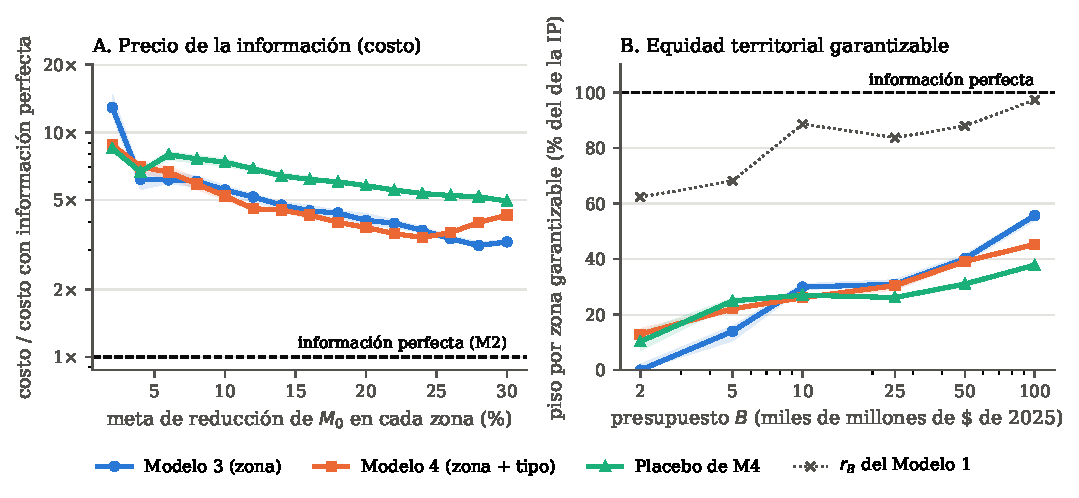
\includegraphics[width=\textwidth]{precio_informacion_12nov}
\caption{El precio de la información, con la equidad territorial de los
Modelos 1 y 2. A: costo de reducir $\Mcero$ en cada zona relativo al costo con
información perfecta (escala logarítmica). B: piso por zona máximo garantizable
como porcentaje del que se garantizaría con información perfecta y el mismo
presupuesto; la línea punteada es el $r_B$ del Modelo 1. Líneas: mediana de las
réplicas; bandas: IC del 95\,\% por \emph{bootstrap}.}
\label{fig:precio}
\end{figure}

Los dos criterios cuentan la misma historia.

\paragraph{1. No saber quién es pobre es caro.} Con metas de hasta el 10\,\% en
cada zona, el Estado que focaliza solo por zona gasta entre \zMtresIPbaja{}
veces lo necesario. El costo de la falta de información es mayor justo donde
están los programas reales, que tienen presupuestos acotados y metas modestas.
Con metas grandes la brecha se reduce, aunque no desaparece: el M3 sigue
costando entre \zMtresIPalta{} veces lo necesario.

\paragraph{2. Sin información individual no se puede prometer la equidad
territorial del Modelo 1.} Con el piso $r_B$ que el Modelo 1 cumple con
información perfecta, M3 y M4 son infactibles en todas las réplicas. El piso
máximo que pueden garantizar va de casi nada con $B=\$2$~mm a entre el 45 y el
56\,\% del de la información perfecta con $B=\$100$~mm (panel B), siempre por debajo de
$r_B$. Un Estado que no sabe quién es pobre no solo gasta más: tampoco puede
asegurar que la reducción de la pobreza llegue a cada zona en la proporción que
podría con información perfecta.

\paragraph{3. La información demográfica vale casi lo mismo que la geográfica.}
Con la meta en cada zona, el M4 cuesta algo menos que el M3 en las metas del 10
al 24\,\% (entre un 4 y un 11\,\% menos), lo mismo en las del 4 al 8\,\% y más en
las del 26 al 30\,\%, y entre un \zPlacMin{} y un \zPlacMax{} menos que un placebo con su
misma partición. La comparación con el placebo muestra que los tipos de
hogar sí contienen información útil, pero que con exigencias territoriales esa
información solo compensa lo que se pierde al no focalizar los indicadores
privados por zona. Sin exigencias territoriales (la sensibilidad de la
Sección~\ref{sec:res34}) la conclusión es otra: el M4 es más barato que el M3,
pero hasta metas del 18\,\% igual de barato que el placebo, de modo que su
ventaja viene de usar celdas más finas.

\paragraph{4. La diferencia es solo de información.} Con un hogar por celda, el
M3 reproduce el costo del M2 con la meta en cada zona y las personas del M1 con
el piso $r_B$, salvo la desviación acotada del ciclo de educación para adultos
(Sección~\ref{sec:diseno}). Por eso las brechas de la Figura~\ref{fig:precio} no
se deben a que los modelos sean distintos: miden el valor de la información
sobre quién es pobre.

% Responsable: Jerónimo (interpretación); Martín agrega lo de M1/M2
% Tesis: la brecha M2 -> M3 es el costo de no saber quién es pobre; M4 recupera
% parte, pero con presupuesto bajo esa ganancia es de la partición, no de la demografía.
\section{Discusión}\label{sec:discusion}

\pendiente{Interpretación del precio de la información para la política pública.}

\pendiente{Cuándo suma la demografía (B $\ge$ 50 mm) y cuándo es solo la partición
(B $\le$ 25 mm, M4 $\approx$ placebo).}

\pendiente{Limitaciones: supuestos del paper (independencia de indicadores, costo
marginal constante), costos provisionales, horizonte de un año.}

% Responsable: AMBOS (lunes en la noche)
\section{Conclusiones}\label{sec:conclusiones}
\pendiente{3--4 hallazgos, recomendación de política y trabajo futuro.}


\bibliographystyle{plainnat}
\bibliography{refs}

\appendix
% Responsable: Martín (Lin 1-5, M1/M2) y Jerónimo (Lin 6-10, M3/M4)
\section{Linealización con Big-M}\label{app:lin}

\subsection{Condiciones de pobreza (Modelos 1--4)}
\pendiente{Martín: Lin 1--5 en la versión del M1/M2. En M3/M4 son
\eqref{eq:m3-r4}--\eqref{eq:m3-r6}.}

\subsection{Mecanismo de cobertura (Modelos 3--4)}

Para cada par activo $(i,j)$, con $M_{ij}=1$, \citet[Apéndice~1]{hamie2024}
introducen las binarias $b2_{ij}$ y $b3_{ij}=1-b2_{ij}$ y escriben la
implicación~\eqref{eq:m3-sorteo} como
\begin{align}
\Ndec_{ij} &\le \mathrm{M}\, b2_{ij}, \tag{Lin 6}\\
\cob_{jd_i} - R_{ij} &\le -\varepsilon + \mathrm{M}\,(1-b2_{ij}), \tag{Lin 7}\\
\Ndec_{ij} + \mathrm{M}\, b3_{ij} &\ge M_{ij}, \tag{Lin 8}\\
\Ndec_{ij} - \mathrm{M}\, b3_{ij} &\le M_{ij}, \tag{Lin 9}\\
R_{ij} - \cob_{jd_i} &\le \mathrm{M}\, b2_{ij}. \tag{Lin 10}
\end{align}
En el paper, Lin~7 es estricta ($\cob<R$). La escribimos con
$\varepsilon=10^{-6}$, el mismo valor que en~\eqref{eq:m3-autoconsistente}: si
cambia uno, tiene que cambiar el otro.

\paragraph{Verificación rama por rama.}
\begin{itemize}
\item $b2_{ij}=0$ ($b3_{ij}=1$): Lin~6 da $\Ndec_{ij}=0$ y Lin~10 da
  $R_{ij}\le\cob_{jd_i}$. Lin~7, 8 y 9 quedan holgadas. Es la rama ``el hogar
  sale de la privación''.
\item $b2_{ij}=1$ ($b3_{ij}=0$): Lin~8 y Lin~9 dan $\Ndec_{ij}=M_{ij}=1$ y Lin~7
  da $\cob_{jd_i}\le R_{ij}-\varepsilon$. Lin~6 y 10 quedan holgadas. Es la rama
  ``sigue privado''.
\end{itemize}
Las dos ramas cubren todos los casos y no se solapan, así que la linealización
es correcta. Como $\Ndec$, $M$, $\cob$ y $R$ están todos en $[0,1]$, basta
$\mathrm{M}=1$ en las cinco restricciones. Con ese valor, en los pares activos
$\Ndec_{ij}=b2_{ij}$ idénticamente, de modo que $b2$ y $b3$ se pueden eliminar.
En los pares con $M_{ij}=0$ no hace falta variable, porque $\Ndec_{ij}=0$. Así
la formulación directa queda con una binaria por par activo
(\cParesActivos{}). La reformulación por cortes
(Proposición~\ref{prop:cortes}) reemplaza también esas binarias.

% Responsable: Jerónimo (M3/M4); Martín agrega filas de M1/M2
% Fuente: docs/desviaciones-paper-m34-6nov.md (18 filas)
\section{Desviaciones respecto a Hamie, Hlasny y Jouni (2024)}\label{app:desv}
\pendiente{Tabla: qué hace el paper, qué hacemos, por qué y efecto medido.}

% Responsable: Martín
% Fuente: docs/informe_modelo1.md §6.8, Modelos/parametros.py
\section{Costos por indicador}\label{app:costos}
\pendiente{Tabla de $\EpF_j$ con fuente oficial y unidad de pago.}


\end{document}
